% !TEX root = catron-dissertation.tex
\epstopdfsetup{outdir=./images/04_dispersion_analysis/}

\chapter{Dispersion Analysis}
Dispersion analysis is an expansion of power spectra analysis from one-dimension to $n$-dimensions.
The technique allows a signal that is measured in both time and space to be separated into not only temporal-frequency components but also spacial-frequency components.
This allows not only the direction of travel that a particular wave to be determined but also the velocity of which that the wave travels.
The benefits of using a dispersion analysis are shown in Figure \ref{fig:04_dispersion_demo}.
\begin{figure}
\centering
  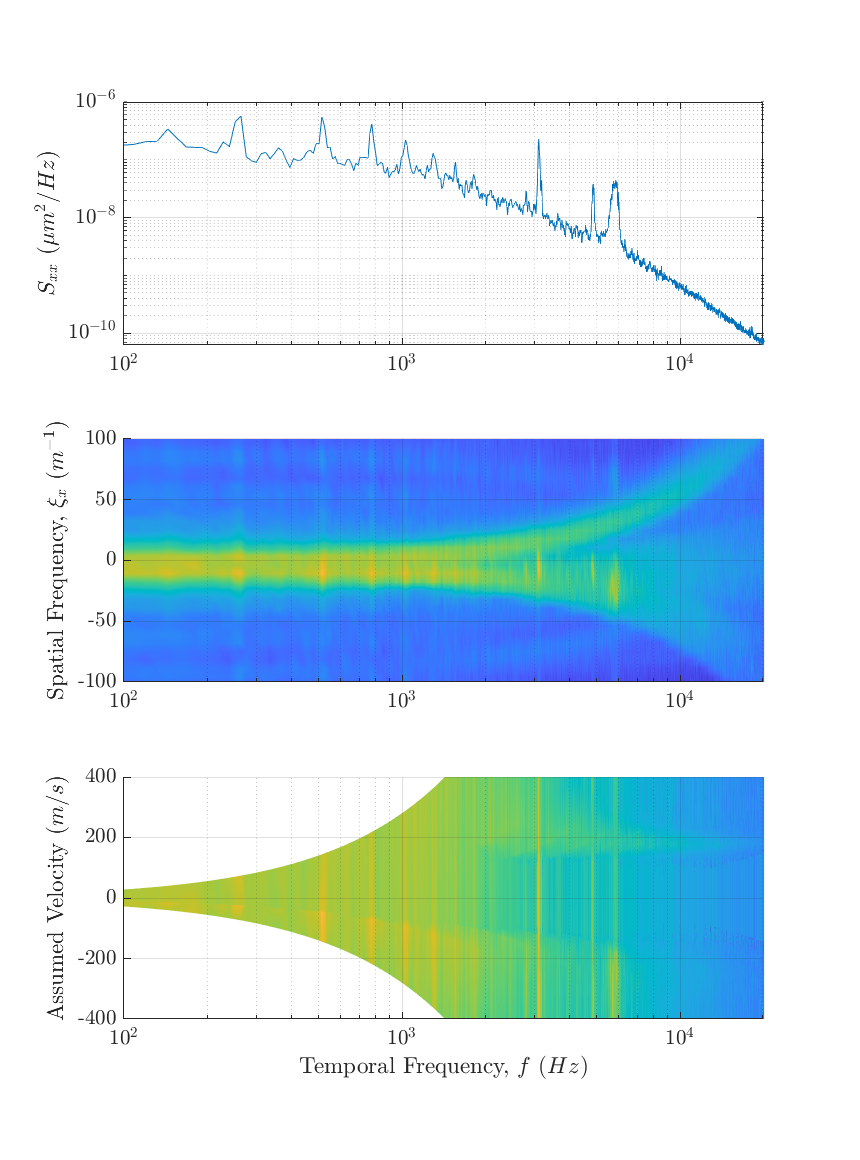
\includegraphics{../matlab/04_dispersion_analysis/dispersion_demo.eps}
  \caption{Dispersion plot example and comparison to traditional power spectra measurements. A single row of a wavefront measurement was used in this example. The top plot shows the typical power spectra measurement averaged over the entire row of data. Both the middle and bottom plots show the dispersion plot with the y-axis as spacial-frequency in the middle and velocity in the bottom assuming $u=f/\xi_x$.}
  \label{fig:04_dispersion_demo}
\end{figure}
The single row of sub-apertures from a wavefront measurement conducted with a 5-inch diameter beam propagating normally through two boundary layers with a free-stream Mach number of 0.5.
This measurement was preformed in the University of Notre Dame Whitefield Wind Tunnel in a test section that contained a model representing the fuselage of the AAOL aircraft \cite{Jumper-2013-8KtN3pue} with window that was flat and flush to the outer mold line of the fuselage.
The top plot shows a traditional power spectra representation averaged over the row of data.
Both the blade-passing frequency (517-Hz) and its sub-harmonic had similar power levels with an additional five harmonics showing significant spikes above the local baseline measurement.
There are three additional strong peaks at approximately 3100, 4850, and 5850 Hz that do not have an easily identifiable source or explanation.

Both the middle and bottom plots show a dispersion plot or two-dimensional power spectra measurement.
The colorbars were intentionally not shown in order to allow for all three plots to be aligned in the temporal frequency axis and the color space is representative of the power spectra in log-space.
The middle plot shows horizontally moving waves with the y-axis representing the spatial frequency, $\xi_x$, with units of inverse meters.
Waves with positive spatial frequencies are moving in the direction of flow.
All of the temporal frequency below 2000-Hz where the is an obvious separation between the upstream and downstream traveling optical disturbances are significantly more on the upstream traveling side.
The blade-passing frequency and its various harmonics show some significant broadband spatial frequency signals.
The three signals of unknown origin are clearly moving upstream but also show some significant broadband spatial signal that is indicative of a source producing optical disturbances that travel in both directions around the tunnel similar to the blade-passing frequency disturbances coming off of the wind tunnel fan.
In addition to optical disturbances branching off in the upstream and downstream moving directions there is a significant disturbances along zero spatial frequency representing a collection of standing waves.

The bottom plot shows the same dispersion plot as the middle one but with the y-axis representing an assumed velocity, $u_{assumed}$, where
\begin{equation}
  u_{assumed} = \frac{f}{\xi_x} \textrm{.}
  \label{eqn:04_velocity_assumed}
\end{equation}
The actual velocity, $u$, of a disturbance in the dispersion plot would be
\begin{equation}
  u = \frac{\partial f}{\partial \xi_x} \textrm{.}
  \label{eqn:04_velocity_actual}
\end{equation}
The assumed velocity measurement is in effect a average of the actual velocity assuming a zero-zero intercept in frequency space.
As there was no discernible separation between disturbance the upstream and downstream moving disturbances in the middle plot below 2000-Hz, there is no discernible velocity below that point.
The primary optical disturbance moving in the direction of flow is moving at the free-stream velocity of approximately 175-m/s.
The upstream traveling disturbance is traveling at the same speed but due to the signal being broader is more difficult to measure this way.
When the middle plot is shown with all linear axis, the slope of any given line through the origin is the inverse of the assumed velocity.
This is why the disturbances along the zero-spatial frequency line are a collection of standing waves and not some structure with broadband temporal content as it would be traveling at near infinite speed.
More discussion will follow a derivation of the dispersion analysis technique which is the n-dimensional power spectra.

\section{One-Dimensional Power Spectra Calculation}
The typical power spectra calculation on a set of data is only in one dimension.
This single dimension is often a time as would be the case when measuring a time series from a single sensor.
A sensor array used to take data at one moment in time could used to measure the power spectra in terms of spatial frequencies.
For a typical single-point measurement that varies in time, $x(t)$, the power spectra calculation is
\begin{equation}
 S_{xx} = \frac{|\fft(x(t))|^2}{N\cdot f_{s}} \textrm{,}
 \label{eqn:04_basic_sxx}
\end{equation}
where $\fft$ is the Fast Fourier Transform, $N$ is the number of samples, and $f_{s}$ is the sample rate.
For data that has only a real component the Fast Fourier Transform function produces magnitude and phase relations at each frequency step, $f_{s}/N$, over the range from zero-frequency up to but not including the Nyquist frequency, $f_s/w$, with a mirrored set of data that can be represented either below (starting at $-f_s/2$) or above (ending just below $f_s$) this range.
The Nyquist frequency not being included and the mirrored data is due to an assumption that is integral to the Fourier Transform, that being the signal is assumed to be periodic.

The total energy, $\sigma^2$, of the signal must be preserved through the transform from physical space-time to frequency space
\begin{equation}
  \sigma^2 = \frac{\sum x^2(t)}{N} = \Delta f\sum S_{xx}(f) \textrm{.}
  \label{eqn:04_fft_energy_conservation}
\end{equation}
Additionally, because of the periodic nature of the Fourier Transform and a finite sample length of discrete data, spectral leakage can cause the power in one frequency bin to leak into adjacent frequency bins.
To minimize this spectral leakage, windowing functions are employed which typically force the end points of the signal to zero.
The Hann window,
\begin{equation}
 w(t) = 1/2\left[1-\cos\left(\frac{2\pi t}{T}\right)\right] \textrm{,}
 \label{eqn:04_hann_window}
\end{equation}
is one of the more commonly used windowing functions where $w(t)$ is the window function, $t$ is the time at a given sample, and $T$ is the total sample time.
Since the windowing of a data set changes the signal energy some correction is needed to be applied.
For an arbitrary windowing function the correction factor, $c_w$, can be obtained by substituting the windowing function in place of $x(t)$ in Equation \ref{eqn:04_fft_energy_conservation},
\begin{equation}
 c_w = \frac{1}{\sqrt{\sum w^2(t)/N}} \textrm{.}
 \label{eqn:04_window_correction}
\end{equation}
For a Hann window this correction factor approaches $\sqrt{8/3}$ as $N$ goes to infinity.
When Equation \ref{eqn:04_basic_sxx} is combined with a windowing function and associated correction the double sided power spectra equation in one dimension becomes
\begin{equation}
 S_{xx} = \cdot\frac{|c_w\cdot\fft\{x(t)\cdot w(t)\}|^2}{N\cdot f_{s}} \textrm{.}
 \label{eqn:04_windowed_sxx}
\end{equation}
A simple MATLAB function for computing the power spectra of a one-dimension signal with an arbitrary windowing function is shown in Listing \ref{code:sc_simpleSXX}.

\section{N-Dimensional Power Spectra Calculation}
For measurements with multiple spatial and temporal dimensions the Fast Fourier Transform is just applied $n$-times where $n$ is the total number of dimensions, with each application in a different dimension,
\begin{equation}
 \fftn(x) = \fft(\fft(\cdots\fft(\fft(x,1),2)\cdots,n-1),n) \textrm{,}
 \label{eqn:04_fftn}
\end{equation}
where $\fft(x,n)$ is the Fast Fourier Transform of $x$ in the $n^{th}$ dimension.
For a $n$-dimensional array the power spectra the function becomes,
\begin{equation}
 \mathbf{S_{xx}} =c_w\cdot\frac{|\fftn\{f(\mathbf{x})\cdot w(\mathbf{x})\}|^2}{\prod{\overrightarrow{N}\cdot\overrightarrow{f_s}}} \textrm{,}
 \label{eqn:04_sxxn}
\end{equation}
where $\mathbf{S_{xx}}$ is the $n$-dimensional power spectra array or dispersion array, $f(\mathbf{x})$ is a $n$-dimensional set of data, $w(\mathbf{x})$ is a $n$-dimensional windowing function, $\overrightarrow{N}$ is a vector denoting the number of elements in each dimension, $\overrightarrow{f_s}$ is a vector denoting the sample rate in each dimension, and
\begin{equation}
 c_w = \frac{1}{\sqrt{\sum w^2(\mathbf{x})/\prod{\overrightarrow{N}}}} \textrm{.}
 \label{eqn:04_windown}
\end{equation}
The signal energy conservation relationship becomes
\begin{equation}
  \sigma^2=\frac{\sum\mathbf{x}}{\prod{\overrightarrow{N}}} = \prod{\overrightarrow{\Delta f_s}}\sum\mathbf{S_{xx}} \textrm{,}
  \label{eqn:04_fftn_energy_conservation}
\end{equation}
where $\overrightarrow{\Delta f_s}$ is a vector representing the frequency step sizes in each dimension.
A simple MATLAB code for calculating the dispersion of $x$ with an arbitrary windowing function is shown in Listing \ref{code:sc_simpleSXXn}.

\section{Non-Rectangular Spatial Windows}
For n-dimensional data sets that fill a rectangular array, a windowing function can easily be created by multiplying together a series of one-dimensional windowing functions created in the direction of each dimension.
For non-rectangular data sets, such as is often the case with optical wavefront measurement, windowing functions take some additional steps in there construction.
In cases when the spatial measurement locations are constant throughout time, the windowing function can be split into two separate components,
\begin{equation}
 w(\mathbf{x}) = w_t(t)\cdot w_s(x,y) \textrm{,}
 \label{eqn:04_window_sep}
\end{equation}
the temporal windowing function, $w_t(t)$, and the spatial windowing function, $w_s(x,y)$.
This paper uses a Hann window for the temporal windowing function and a modified Hann window for the spatial windowing function.
For the case of a circular aperture, the Hann window can be reformulated to be based normalized radius, $\rho_N$, of the aperture,
\begin{equation}
 w_s(\rho_N) =
 \begin{cases}
  \frac{1+\cos(\pi\cdot\rho_N)}{2} & \textrm{if } \rho_N < 1 \\
  0                                & \textrm{otherwise.}
 \end{cases}
 \label{eqn:04_window_space}
\end{equation}
This modified Hann window is two-dimensional with a value of one at the center of the aperture and decreases to zero at the edge of the aperture in the same manor as a Hann windows decreases from the center to either end.

Because the wavefronts used often had a clipped edge or other obscuration a different method was actually employed.
For an arbitrary shaped aperture, the minimum distance from any given measurement location to the edge of the aperture is used to create the spatial windows.
The minimum distance can be computed given the a set of points ($x$ and $y$) that spans the measurement range and the set of points outside of the aperture ($x_O$ and $y_O$),
\begin{equation}
 d_{min}(x,y) = \min\left\{\sqrt{(x-x_{O})^2+(y-y_{O})^2}\right\} \textrm{.}
 \label{eqn:04_window_space_arb_dist}
\end{equation}
This distance is then normalized by the maximum value and the resulting spatial window given a modified Hann window,
\begin{equation}
 w_s(x,y) = \frac{1+\cos\left\{\pi\cdot\left(1-d_{min}^{norm}(x,y)\right)\right\}}{2} \textrm{.}
 \label{eqn:04_window_space_arb}
\end{equation}
This same basic process can be extended to data sets where the locations of measurements in space vary with time.

\section{Dispersion Analysis}
At the beginning of this chapter a dispersion plot was shown along with a typical power spectra plot in Figure \ref{fig:04_dispersion_demo}.
This was for the purpose of doing a simple discussion of on some of the benefits of using a dispersion analysis on optical wavefronts.
That simple analysis was using only a single row of a wavefront and provided an incite into the disturbances that were moving in the horizontal direction only.
When a dispersion analysis is performed over all dimensions of a wavefront, as will be done for the remained of the chapter additional detail is available, additional detail as well as determination of optical disturbances moving vertically or any direction in between.
Figure \ref{fig:04_dispersion_xy} shows both the horizontally and vertically moving optical disturbances.
\begin{figure}
  \centering
  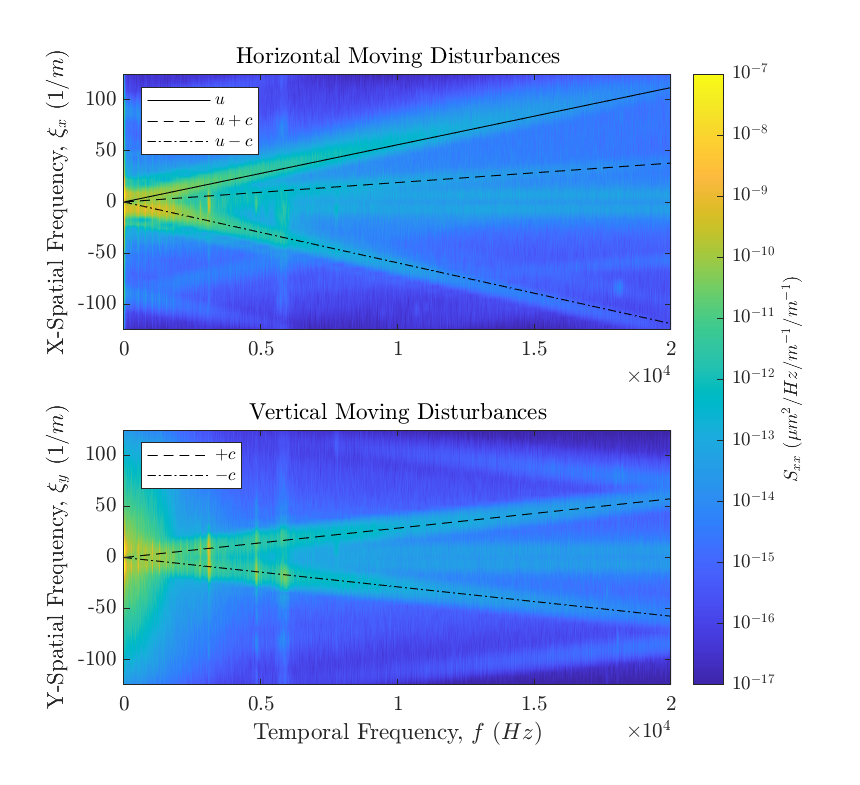
\includegraphics{../matlab/04_dispersion_analysis/dispersion_xy.eps}
  \caption{Horizontal and vertical moving optical disturbances. This is the same data as presented in Figure \ref{fig:04_dispersion_demo} but after calculating the full three-dimensional power spectra. The horizontal disturbances are shown at zero vertical spatial frequency and likewise the vertical disturbances are shown at zero horizontal spatial frequency.}
  \label{fig:04_dispersion_xy}
\end{figure}
The top plot shows the horizontally moving disturbances and when compared to the similar plot as shown in Figure \ref{fig:04_dispersion_demo} additional detail can be observed.
This is partially due to the significant increase in spatial information but also due to the two-dimensional dispersion averages together information in the vertical direction.


\begin{figure}
  \centering
  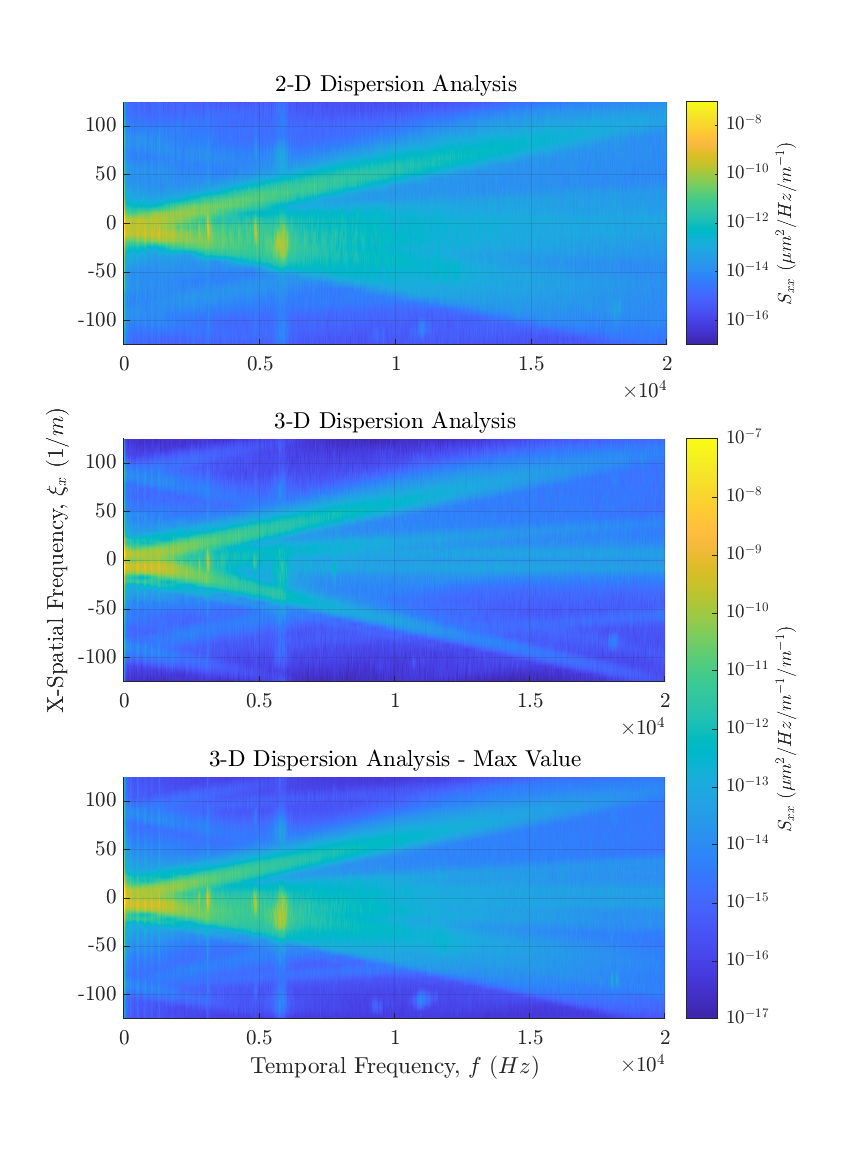
\includegraphics{../matlab/04_dispersion_analysis/dispersion_comparison.eps}
  \caption{Horizontal moving optical disturbances comparison. The top plot shows a two-dimensional dispersion analysis over a single row of data. The middle plot shows a three-dimensional dispersion analysis at $\xi_y=0$. The bottom plot shows the same three-dimensional dispersion analysis but showing the maximum value through the vertical axis.}
  \label{fig:04_dispersion_comparison}
\end{figure}




\begin{figure}
  \centering
  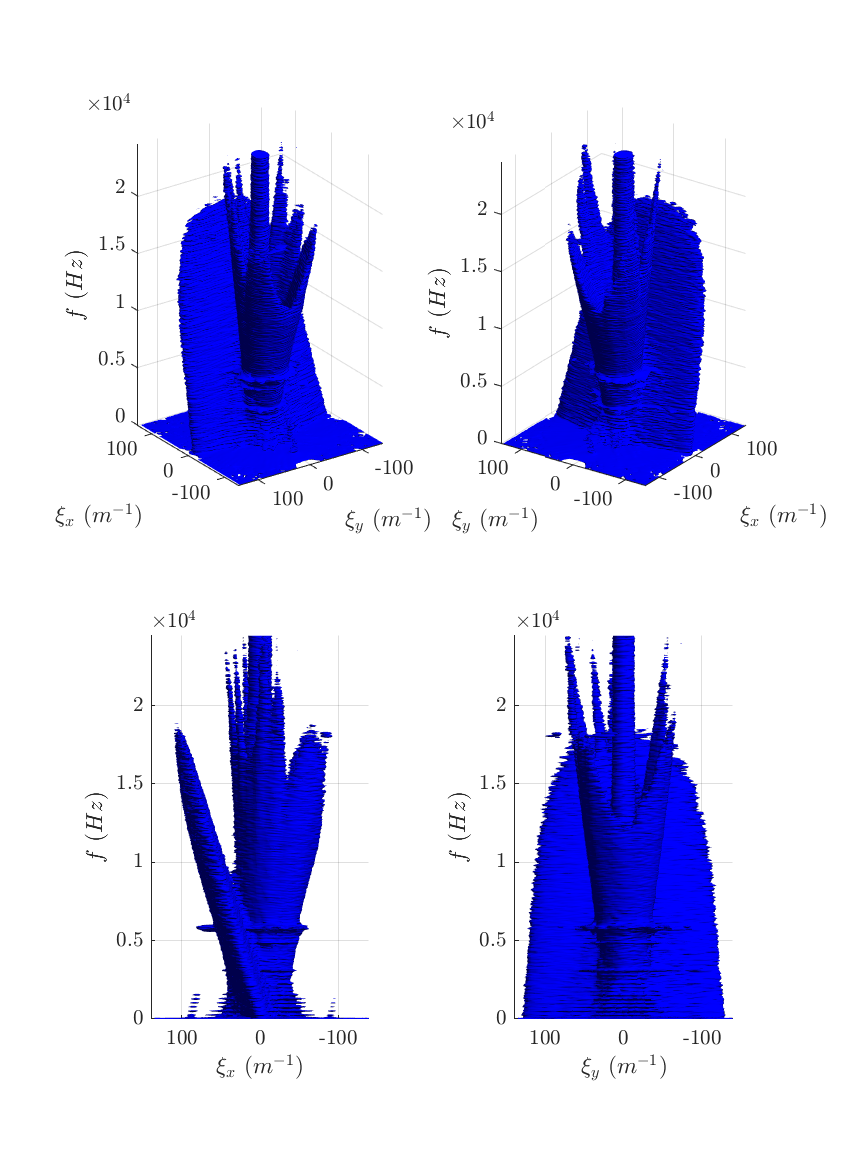
\includegraphics{../matlab/04_dispersion_analysis/dispersion_3d.eps}
  \caption{Three-dimensional view of the dispersion plot showing an isosurface at a power of $10^{-14}$ $\mu m^2/Hz/m^{-1}/m^{-1}$. The isosurface encompasses 99.9\% of the power of the wavefront.}
  \label{fig:04_dispersion_3d}
\end{figure}

\begin{figure}
  \centering
  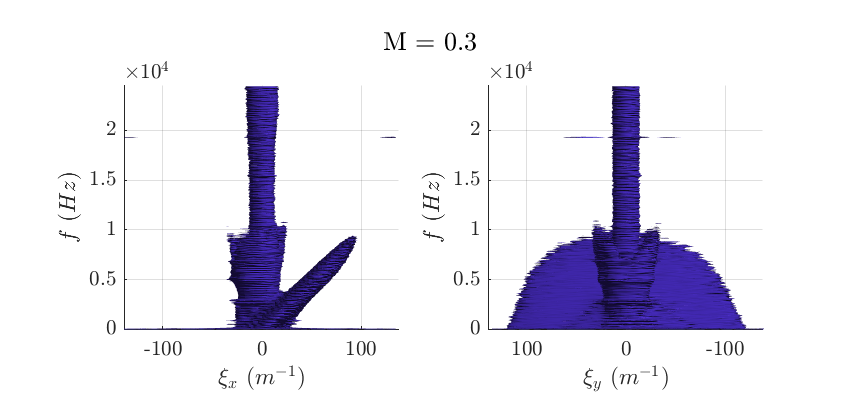
\includegraphics{../matlab/04_dispersion_analysis/dispersion_mach_0.3.eps}
  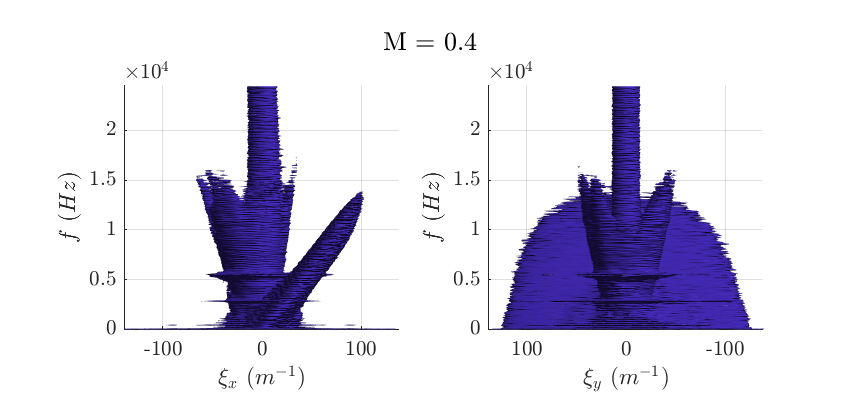
\includegraphics{../matlab/04_dispersion_analysis/dispersion_mach_0.4.eps}
  \includegraphics{../matlab/04_dispersion_analysis/dispersion_mach_0.5.eps}
  \caption{Three-dimensional view of dispersion plots as the Mach number increased from 0.3 to 0.5. The isosurfaces are all shown at a power of $10^{-14}$ $\mu m^2/Hz/m^{-1}/m^{-1}$ and all encompass 99.9\% of the wavefront power.}
  \label{fig:04_dispersion_mach}
\end{figure}
